% -*- mode: fundamental -*-

% ****************************************************************

\chapter{BSV Combinational circuits for the RISC-V Decode step}

\markboth{Ch \arabic{chapter}: Combinational Decode (DRAFT)}{\copyrightnotice}

\setcounter{page}{1}
% \renewcommand{\thepage}{\arabic{page}}
\renewcommand{\thepage}{\arabic{chapter}-\arabic{page}}

\label{ch_Combo_Circuits}

% ****************************************************************

\section{Introduction}

In this chapter we focus on learning enough BSV to write code for the
Decode step of the RISC-V interpretation steps shown in
Figure~\ref{Fig_Simple_Instr_Exec}.  As mentioned earlier, we choose
to start with the Decode step (instead of the Fetch step) to
facilitate the BSV-learning process.

The inputs to the Decode step as depicted in
Figure~\ref{Fig_Simple_Instr_Exec} are:

\begin{tightlist}

 \item A 32-bit piece of data---RISC-V instruction---that has become
 available by reading it from memory at the PC address.\footnote{In
 RISC-V, so-called ``compressed'' instructions can be 16-bits, but we
 ignore that for now}

 \item Any additional information passed on from the Fetch step.

\end{tightlist}

The outputs of the Decode step have information needed by the next
step (Register-Read and Dispatch).  For a RISC-V instruction, useful
information includes:

\begin{tightlist}

 \item Is it a legal 32-bit instruction?

 \item If legal, what is its broad classification: Branch? Integer
   Arithmetic or Logic? Memory Access?  This will help the next step
   in dispatching to one of the Execute steps.

 \item Does it have zero, one or two input registers?  If so, which
   ones?  This will help the next step in reading registers.

 \item Does it have zero or one output registers?  If so, which one?
   This will help the final Register Write step in writing back a
   value to a register.

\end{tightlist}

To compute these values, we need to examine ``slices'' of the 32-bit
instruction (``bit vector''), such as the 7-bit ``opcode'' slice, the
5-bit ``rs1'', ``rs2'' and ``rd'' slices, and so on.  We need to be
able to compare these slices to constants ({\eg} ``Is the opcode a
BRANCH opcode?'').  We need to do things conditionally, {\eg} if it is
a BRANCH instruction, then it has an rs1 and rs2 slice but no rd
slice.  We need to bundle together all these bits of output
information so that we can pass to to the next step, for which we need
some kind of ``struct'' or ``record'' structure.  Finally, as in all
good programming language methodology, we'd like to package up all
this functionality inside a ``function'' with clearly specified
input(s) and output(s).

In the next several sections---\ref{Sec_BSV_Bit_Vectors},
\ref{Sec_BSV_Boolean_values}, \ref{BSV_if_then_else},
\ref{BSV_functions}---we will learn the BSV concepts needed to code
the Decode step.  Then, in Section~\ref{Sec_Combo_Decode} we use these
concepts to show the BSV code for the Decode function.

% ****************************************************************

\section{BSV: Bit Vectors}

\label{Sec_BSV_Bit_Vectors}

\index{BSV!Bit Vectors}
\index{BSV!Types!Bit\#(n)}

In BSV, as in many programming languages, every value has a
\emph{type}.  The simplest, and lowest-level type in BSV is the
bit-vector (a vector made up of a particular number bits).  Later we
will see that in BSV one can define more abstract types such as
integers, booleans, vectors and arrays, lists, structs (records),
tagged unions (algebraic types), trees, and so on.  However,
ultimately, any such value is represented in hardware as a bit-vector.

The BSV statement:

\begin{Verbatim}[frame=single, numbers=left]
   Bit #(32) pc_val;
\end{Verbatim}

declares the identifier \verb|pc_val| to have the type
\verb|Bit#(32)|, {\ie} a bit-vector of 32 bits.
The general syntax is similar to C or Verilog:
\begin{quote}
\emph{type} \emph{identifier};
\end{quote}

The BSC type \verb|Bit#(32)| is roughly equivalent to the C type
\verb|uint32_t|.  Unlike C, where only a few sizes are available, all
multiples of 8 bits--- (\verb|uint8_t|, \verb|uint16_t|,
\verb|uint32_t| and \verb|uint64_t|)---bit-vectors in BSV can have any
size (\verb|Bit#(3)|, \verb|Bit#(51)|, \verb|Bit#(512)|, ...).

The bits in a BSV bit-vector of size $n$ are indexed from $n-1$
(most-significant bit) to 0 (least-significant bit).  You can extract
a \emph{slice} of a bit-vector using usual Verilog notation:

\index{BSV!Bit Vectors!slices}

\begin{Verbatim}[frame=single, numbers=left]
   Bit #(32) pc_val;
   Bit #(12) page_offset = pc_val [11:0];
\end{Verbatim}

In the second line, we extract 12 bits of \verb|pc_val| to get a
bit-vector of size 12.  BSV is \emph{strongly typed} with respect to
sizes, {\ie} it is very strict about matching sizes.  For example,
this statement:

\begin{Verbatim}[frame=single, numbers=left]
   Bit #(12) page_offset = pc_val [10:0];
\end{Verbatim}

will be reported as a type-error by the \emph{bsc} compiler because
the slice-expression on the right-hand side has type \verb|Bit#(11)|
which does not match the declared type \verb|Bit#(12)|.

BSV bit-vectors can be compared for equality and inequality.  BSV
bit-vectors are synonymous with unsigned integers, and so a number of
other operations are also available on bit-vectors.  Examples:

\index{BSV!Bit Vectors!operators}

\begin{Verbatim}[frame=single, numbers=left]
   Bit #(12) x, a, b, c, d, e, f;

   // Comparison ops: result type is Bool
   if (a == b) ...;        // equality
   if (a != b) ...;        // not-equal to
   if (a < b) ...;         // less-than
   if (a <= b) ...;        // less-than-or-equal-to
   if (a > b) ...;         // greather-than
   if (a >= b) ...;        // greater-than-or-equal-to

   // Arithmetic ops: result type is Bit #(12)
   x = a + b - c * d;      // add, subtract, multiply

   // Bitwise logic ops: result type is Bit #(12)
   //   AND  OR   unary INVERT   XOR  XNOR  XNOR
   x = a &  b |     (~ c)         ^   d ^~ e ~^ f;

   // Shifts
   x = (a << 3) & (b >> 14);    // left- and right-shift
\end{Verbatim}

Please see the \emph{BSV Language Reference Guide}~\cite{BLang2000},
Section 10.3, ``Unary and binary operators'' for a full list of
available unary and binary operators.  Unlike Haskell, in BSV you
cannot define new unary or binary infix operators.

In such expressions, as usual bit-vector sizes must match exactly,
else we'll get a type error, {\eg} we cannot compare a
\verb|Bit#(12)| value with \verb|Bit#(11)| value.  Unlike C and
Verilog, BSV does not implicitly extend or truncate bit-vectors to
match sizes.

\index{BSV!Bit Vectors!truncate}
\index{BSV!Bit Vectors!extend}
\index{BSV!Bit Vectors!zeroExtend}

Two functions are available to zero-extend and truncate bit-vectors.
\begin{Verbatim}[frame=single, numbers=left]
   Bit #(12) a;
   Bit #(10) b;
   b = a;                         // Type error: mismatched sizes
   a = b;                         // Type error: mismatched sizes
   b = truncate (a);              // Ok; truncates a to Bit #(10), then assigns
   a = zeroExtend (b);            // Ok; extends b to Bit #(12), then assigns
   if (a == zeroExtend (b)) ...   // Ok
   if (truncate (a) < b) ...      // Ok
\end{Verbatim}

The functions \verb|truncate()| and \verb|zeroExtend()| are
\emph{polymorphic} in that they will truncate/extend by the
appropriate amount as demanded by the context.

% ****************************************************************

\section{BSV: Boolean values}

\label{Sec_BSV_Boolean_values}

\index{BSV!Bool}
\index{BSV!Types!Bool}
\index{BSV!Bool!operators}

In BSV, \verb|Bool| is the type of a Boolean value. It has the usual
boolean operators \verb|&&| (Boolean/logical AND), \verb'||'
(Boolean/logical OR) and \verb|!| (Boolean/logical NOT).

% ================================================================

\subsection{BSV: Caution: {\tt Bool} and {\tt Bit\#(1)} are different types}

BSV is unlike languages like C and Python which are very loose about
what can be used as a boolean value.  For example in C, any non-zero
numeric value or pointer is considered ``True''.

In BSV, \verb|Bool| and \verb|Bit#(1)| are \emph{distinct} types,
{\ie} \emph{bsc}'s type-checking will complain if one is used where
the other is expected.  This is because not all \verb|Bit#(1)| values
are meaningful as Boolean values.

The Boolean/logical operators mentioned above (such as \verb|&&|)
operate on \verb|Bool| types and are distinct from the bit-wise logic
operators mentioned earlier (such as \verb|&|), which operate on
\verb|Bit#(n)| types.

Note that bitwise comparison operators, such as in the example
\verb|if (a <= b) ...| shown in Section~\ref{Sec_BSV_Bit_Vectors}
above, take \verb|Bit#(n)| arguments and produce \verb|Bool| results.

% ================================================================

\subsection{BSV: Example: recognizing legal RISC-V BRANCH instructions}

The RISC-V ISA has a family of six conditional-branch instructions.
Figure~\ref{Fig_Combo_BRANCH_instrs} is an excerpt from the Unprivileged ISA
specification document~\cite{RISCV_Unpriv_2019_12_13}.
\begin{figure}[htbp]
  \centerline{
\includegraphics[width=6in,angle=0]{ch040_Combo_Circuits/Figures/Fig_Combo_BRANCH_instrs_1}}
  \centerline{
\includegraphics[width=6in,angle=0]{ch040_Combo_Circuits/Figures/Fig_Combo_BRANCH_instrs_2}}
  \vspace{2mm}
  \centerline{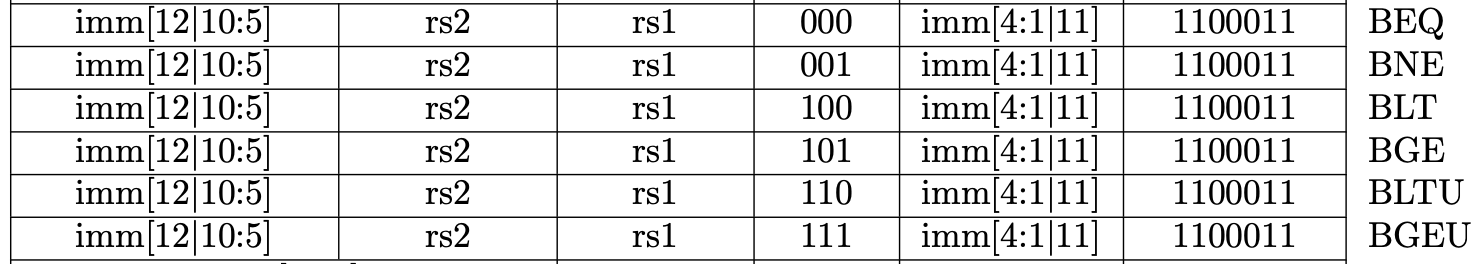
\includegraphics[width=6in,angle=0]{ch040_Combo_Circuits/Figures/Fig_Combo_BRANCH_instrs_3}}
  \caption{\label{Fig_Combo_BRANCH_instrs}RISC-V conditional BRANCH instructions}
\end{figure}
The first line just gives us the names of the various slices of a
32-bit BRANCH-type instruction, and the subsequent lines describe the
six instructions.  Note that they only differ in the \verb|funct3|
slice, where they use only six of the possible eight 3-bit codes.

Assuming \verb|instr| is a 32-bit instruction, we can write BSV code
to compute whether \verb|instr| is or is not a legal BRANCH
instruction:

\begin{Verbatim}[frame=single, numbers=left]
   Bit #(7) opcode_BRANCH = 7'b_110_0011;

   Bit #(7) opcode = instr [6:0];
   Bit #(3) funct3 = instr [14:12];
   Bool legal = (opcode == opcode_BRANCH)
                 && (funct3 != 3'b010)
                 && (funct3 != 3'b011));
\end{Verbatim}

Line 1 defines \verb|opcode_BRANCH| as a 7-bit constant whose binary
value is 1100011.  The \verb|`7b| prefix indicates that the number
should be read as a binary, not decimal, number.  The ``\verb|_|''
underscore characters are present merely for our (human) readability,
and have no semantic significance.  Lines 3-4 extract relevant slices,
and finally lines 5-7 define the desired legality condition.

Figure~\ref{Fig_Combo_Is_Legal_BRANCH} shows the hardware circuit described by the code.
\begin{figure}[htbp]
  \centerline{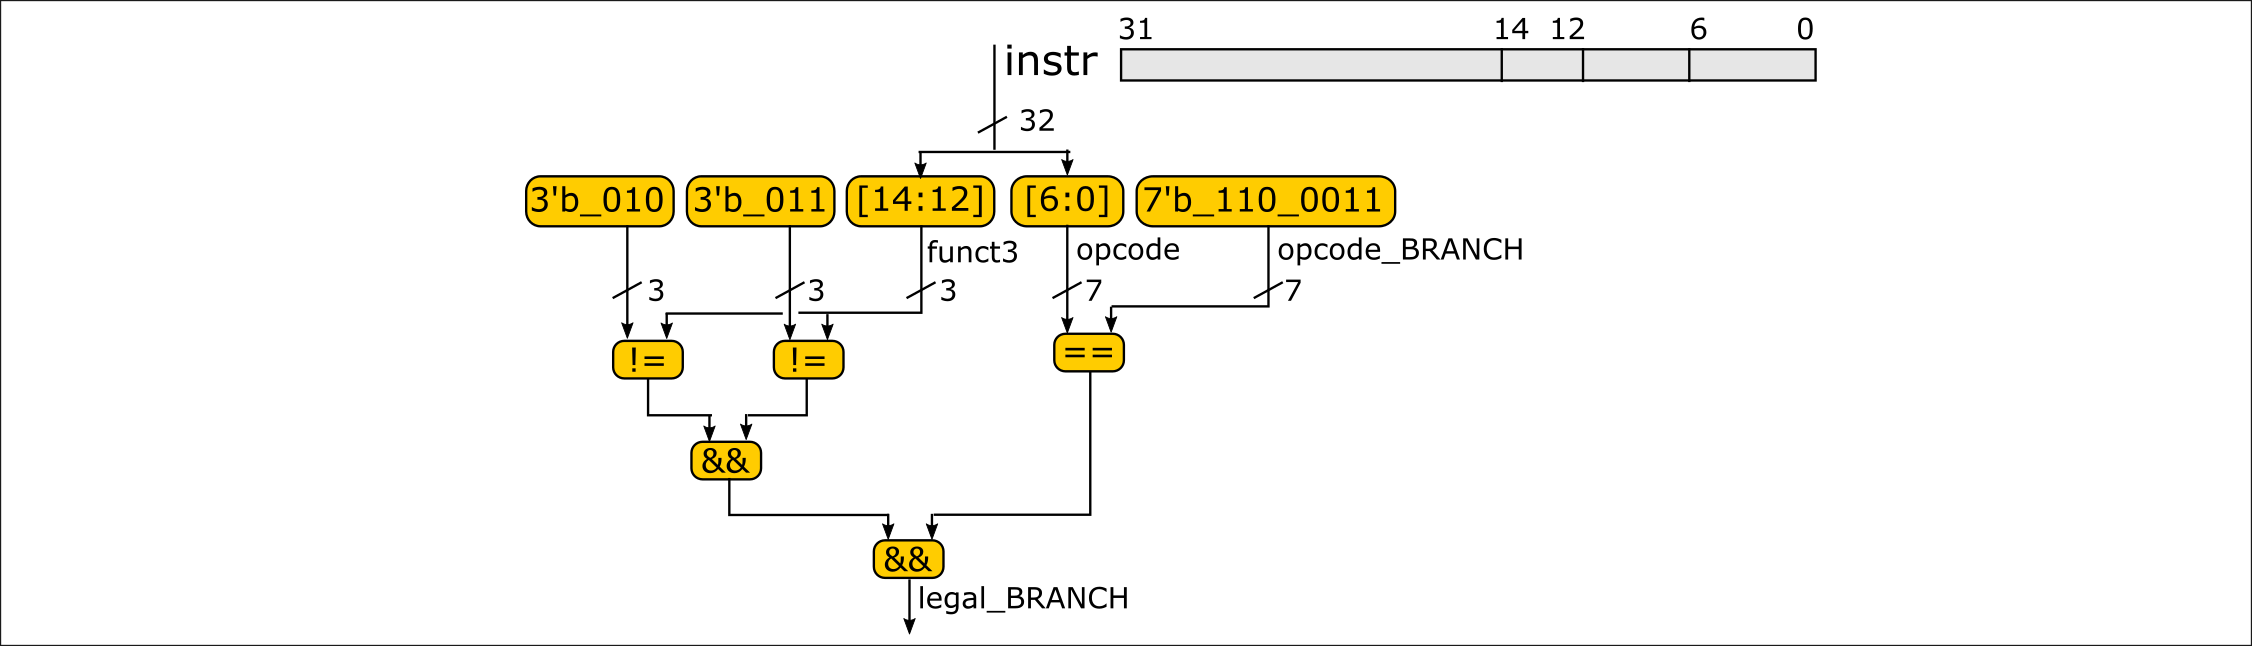
\includegraphics[width=6in,angle=0]{ch040_Combo_Circuits/Figures/Fig_Combo_Is_Legal_BRANCH}}
  \caption{\label{Fig_Combo_Is_Legal_BRANCH}Testing for a legal BRANCH instruction}
\end{figure}
Some observations:
\index{BSV!bus (hardware, bundle of wires)}
\begin{tightlist}

 \item Lines with arrow-heads in the figure represent bundles of one
   or more wires, also called ``buses''.  For buses that have more
   than one wire, we show a small diagonal cross-hatch labeled with
   the number of wires (such as ``3'' or ``7'').

 \item Names/identifiers in BSV code that are bound to values are
   simply names for buses (in most software programming languages
   names represent memory locations; this is \emph{not} the case in
   BSV).

\end{tightlist}

% ================================================================

\subsection{BSV: Combinational circuits and primitives}

\index{BSV!Combinational circuits}
\index{BSV!Combinational primitives}

Figure~\ref{Fig_Combo_Is_Legal_BRANCH} is an example of a so-called
\emph{combinational} circuit.  In general, a combinational circuit is
any interconnection of combinational primitive ``operators'' that
\emph{does not contain cycles} ({\ie} a bus connecting back to an
earlier part of the circuit).  Examples of combinational primitive
operators in BSV include comparisons (like \verb|==| and \verb|!=|),
boolean operations (like \verb|&&|), bit-slicing (\verb|[n1:n2]|)
truncation and extension, arithmetic (like \verb|+|, \verb|-|,
\verb|*|), shifts (\verb|<<| and \verb|>>|), and multiplexers
(discussed in Section~\ref{BSV_if_then_else}, later).

In BSV, and Verilog/SystgemVerilog RTL, we consider such operators as
``primitive''.  In fact, such operators must themselves be implemented
using lower-level circuit primitives such as AND, OR, and NOT gates
which, in turn, must be implemented with even lower-level circuit
structures such as transistors.  We do not concern ourselves with such
lower-level implementation because nowadays this is performed for us
automatically by excellent so-called ``synthesis'' tools.

% ----------------------------------------------------------------

\subsubsection{BSV: Combinational circuits have no side-effects (are ``pure'')}

\index{BSV!Combinational circuits!purity}

There is no ``storage'' in a combinational circuit, nor any concept of
``updating'' any storage (no ``side-effects'').  When a 32-bit value
is presented at the input (top) of the circuit in
Figure~\ref{Fig_Combo_Is_Legal_BRANCH}, conceptually we
``instantly'' see the 1-bit result at the output (bottom) of the
circuit, {\ie} a combinational circuit is conceptually a pure,
instantaneous, mathematical function from intputs to outputs.  If we
change the 32-bit value presented at the input, conceptually the
output changes instantaneously in response.

\index{BSV!Propagation delay}

Note: \fbox{
\begin{minipage}{5in}\small

Circuits are physical artefacts and we cannot escape
physics. Electrical signals will take some finite time to propagate
from inputs to outputs through wires and silicon. This propagation
delay will place a limit on the ``clock speed'' at which we are able
to run a digital circuit.  We ignore this for the moment, and discuss
this in detail later.

\end{minipage}}


% ================================================================

\subsubsection{BSV: Data types identify combinational circuits}

\index{BSV!Combinational circuits!data types}
\index{BSV!Types!Combinational circuits}

In BSV, the output type of any circuit that produces a value will have
one of three forms (the latter two will be discussed in detail later):

\begin{itemize}

\item \emph{... some value type ...}: \verb|Bit#(n)|, \verb|Bool|, or
types discussed later such as structs, enums, tagged unions, vectors,
and so on.

\item \verb|Action|

\item \verb|ActionValue #(| \emph{... some value type ...} \verb|)|

\end{itemize}

Circuits whose output types are of the first form are
\emph{guaranteed} by BSV's type-checking system to be pure
combinational circuits---they cannot have any side-effects such as
updating a register or memory location, enqueuing or dequeuing from a
FIFO, outputting a value to a device or display, {\etc} Circuits with
\verb|Action| and \verb|ActionValue#()| types, on the other hand, may
have side-effects as part of the process of producing their output
value.

\index{BSV!Haskell similarity}

BSV is unusual amongst programming languages in precisely tracking
``pure'' (no side-effects) \emph{vs.} ``impure'' constructs through
type-checking.  In this regard it is most similar to Haskell, where
potentially impure expressions must have certain monadic types
(typically in the ``IO monad'').  The importance of tracking purity
will become clear when we discuss rule and method conditions and
scheduling, later.


% ****************************************************************

\section{BSV: Functions}

\label{BSV_functions}

\index{BSV!functions!definition}

The fragment of code shown above can be packaged into a BSV function,
specifying argument(s) with precise types and a precise result type:

\begin{Verbatim}[frame=single, numbers=left]
function Bool is_legal_BRANCH (Bit #(32) instr);
   Bit #(7) opcode_BRANCH = 7'b_110_0011;

   Bit #(7) opcode = instr [6:0];
   Bit #(3) funct3 = instr [14:12];
   Bool legal = ((opcode == opcode_BRANCH)
                 && (funct3 != 3'b010)
                 && (funct3 != 3'b011));
   return legal;
endfunction
\end{Verbatim}

\index{BSV!functions!application}

Functions are invoked using the ``application'' syntax commonly used
in most programming languages:

\begin{Verbatim}[frame=single, numbers=left]
   Bit #(32) x, y;

   Bool result_x = is_legal_BRANCH (x);
   Bool result_y = is_legal_BRANCH (y);
\end{Verbatim}

BSV function definition and application syntax is similar to
SystemVerilog.

% ****************************************************************

\section{BSV: A small testbench to test our code}

\label{BSV_small_testbench}

\index{BSV!Testbenches}

Here is a small program to run our \verb|is_legal_BRANCH()| function on
a few tests:

\begin{minipage}{6.5in}\small
\begin{Verbatim}[frame=single, numbers=left]
import StmtFSM :: *;

function Bool is_legal_BRANCH (Bit #(32) instr);
   ... as shown earlier ...
endfunction

(* synthesize *)
module mkTop (Empty);

   mkAutoFSM (
      seq
	 action
	    Bit #(32) instr_BEQ = {7'h0, 5'h9, 5'h8, 3'b000, 5'h3, 7'b_110_0011};
	    $display ("instr_BEQ %08h => %0d", instr_BEQ,
		      is_legal_BRANCH (instr_BEQ));
	 endaction

	 action
	    Bit #(32) instr_BNE = {7'h0, 5'h9, 5'h8, 3'b001, 5'h3, 7'b_110_0011};
	    $display ("instr_BNE %08h => ", instr_BNE,
		      fshow (is_legal_BRANCH (instr_BNE)));
	 endaction

	 action
	    Bit #(32) instr_ILL_op = {7'h0, 5'h9, 5'h8, 3'b100, 5'h3, 7'b_110_0000};
	    $display ("instr_ILL_op %08h => ", instr_ILL_op,
		      fshow (is_legal_BRANCH (instr_ILL_op)));
	 endaction

	 action
	    Bit #(32) instr_ILL_f3 = {7'h0, 5'h9, 5'h8, 3'b010, 5'h3, 7'b_110_0011};
	    $display ("instr_ILL_f3 %08h => %0d", instr_ILL_f3,
		      is_legal_BRANCH (instr_ILL_f3));
	 endaction
      endseq);

endmodule
\end{Verbatim}
\end{minipage}

For the moment, don't try to understand all these boilerplate
constructs in detail.  Briefly, \verb|mkAutoFSM| is like a sequential
program.  It performs a sequence of four actions.  In each action we
define a 32-bit instruction with standard Verilog bit-concatenation
syntax.  For example, \verb|instr_BEQ| is defined as a 32-bit value by
concatenating a 7-bit hex 0 as an ``immediate'' value, a 5-bit hex 9
for rs2, a 5-bit hex 8 for rs1, a 3-bit 0 for funct3, a 5-bit hex 7
for rd, and a 7-bit binary value for the branch opcode.
\verb|instr_BEQ| and \verb|instr_BNE| are legal branch instruction
encodings.  \verb|instr_ILL_op| is not a legal branch instruction
because it has the wrong 7-bit opcode in the opcode slice.
\verb|instr_ILL_f3| is not a legal branch instruction because it has
an illegal 3-bit value in the funct3 slice.

In each action, the \verb|$display()| prints the instruction in hex
format, and prints the \verb|Bool| result of applying
\verb|is_legal_Branch()| to the instruction.  In two of the
\verb|$display()|s we print the \verb|Bool| value as a decimal integer
(\verb|%0d| format).  In the other two \verb|$display()|s we use
\verb|fshow()| to print booleans as ``\verb|True|'' or
``\verb|False|''.

Suppose this code is in a file \verb|Top.bsv|.  We can now compile,
link and execute the design (in simulation) as follows:

\begin{Verbatim}[frame=single, numbers=left]
# ---- Compile BSV source code
$ bsc -u -sim Top.bsv
checking package dependencies
compiling Top.bsv
code generation for mkTop starts
Elaborated module file created: mkTop.ba
All packages are up to date.

# ---- Link to form a simulation exeutable
$ bsc  -sim  -e mkTop -o ./exe_HW_bsim
Bluesim object created: mkTop.{h,o}
Bluesim object created: model_mkTop.{h,o}
Simulation shared library created: exe_HW_bsim.so
Simulation executable created: ./exe_HW_bsim

# ---- Execute the simulator
$ ./exe_HW_bsim
instr_BEQ 009401e3 => 1
instr_BNE 009411e3 => True
instr_ILL_op 009441e0 => False
instr_ILL_f3 009421e3 => 0
\end{Verbatim}

% ================================================================

\subsection{Exercises}

\begin{enumerate}

\item Extend the testbench to test more 32-bit values with
\verb|is_legal_BRANCH()|.

\item Refer to the ``RV32I Base Instruction Set'' listing in ``Chapter
24 RV32/64G Instruction Set Listings'' in the RISC-V Unprivileged ISA
specification document~\cite{RISCV_Unpriv_2019_12_13}.  It lists 40
RV32I instructions.  Similar to \verb|is_legal_BRANCH()|, write BSV
code for the following functions:

\begin{Verbatim}[frame=single, numbers=left]
   function Bool is_legal_JAL (Bit #(32) instr);
      ... acccepts JAL

   function Bool is_legal_JALR (Bit #(32) instr);
      ... acccepts JALR

   function Bool is_legal_IALU (Bit #(32) instr);
      ... acccepts LUI, AUIPC, ADDI, SLTI, ..., OR, AND

   function Bool is_legal_Mem (Bit #(32) instr);
      ... acepts LB, LH, LW, LBU, LHU, SB, SH, SW
\end{Verbatim}

Ignore FENCE, ECALL and EBREAK instructions; for the moment we'll
treat them as illegal instructions.

\item Extend the testbench to test more 32-bit values with all the
\verb|is_legal_XXX()| functions.

\end{enumerate}

% ****************************************************************

\section{BSV: {\tt enum} types}

\label{BSV_enum_types}

\index{BSV!enum types}

In Figure~\ref{Fig_Simple_Instr_Exec}, in the Register-Read
and Dispatch step, we need to know whether the incoming instruction is
illegal, a control instruction (branch or jump), an integer
arithmetic/logic instruction, or a memory-accessing instruction.  We
could think of coding these ``classes'' using numbers (0 for illegal,
1 for control, 2 for IALU, 3 for Mem), but it is more readable, and
cleaner, to use an ``enum'' type (similar to enum types in
SystemVerilog and C):

\begin{Verbatim}[frame=single, numbers=left]
typedef enum {OPCLASS_ILLEGAL,
	      OPCLASS_CONTROL,    // BRANCH, JAL, JALR
	      OPCLASS_IALU,
	      OPCLASS_MEM }       // LOAD, STORE, AMO
OpClass
deriving (Bits, Eq, FShow);
\end{Verbatim}

This defines a type \verb|OpClass| containing four constants,
\verb|OPCLASS_ILLEGAL|, \verb|OPCLASS_CONTROL| ...

\index{BSV!deriving!Bits}

Because we said ``\verb|deriving(Bits)|'', the \emph{bsc} compiler
will automatically represent them with the obvious codes 0, 1, 2 and 3
in a minimal bit-width (\verb|Bit#(2)|).  For other codings, we would
\emph{not} say ``\verb|deriving(Bits)|'', and we would provide an
explicit mapping function into codes (see ``typeclass instances'',
later).

\index{BSV!deriving!Eq}

Because we said ``\verb|deriving(Eq)|'', the \emph{bsc} compiler will
automatically define the ``equality'' (and ``inequality'') functions
for values of this new type, in the natural and obvious way.  For
other definitions of equality/inequality, we would \emph{not} say
``\verb|deriving(Eq)|'', and we would define equality/inequality as we
wish (see ``typeclass instances'', later).

\index{BSV!deriving!Fshow}

Given a value \emph{v} of type \verb|OpClass|, if we directly print it
({\eg} in a \verb|$display()| statement), it will print its numeric
code (0, 1, ...).  Because we said ``\verb|deriving(FShow)|'', the
\emph{bsc} compiler will automatically define an ``\verb|fshow()|''
function for this type: if we print \verb|fshow(|\emph{v}\verb|)|, it
will print its symbolic name from the enum declaration instead
(\verb|OPCODE_ILLEGAL|, \verb|OPCODE_CONTROL|, ...).

% ****************************************************************

\section{BSV: Syntax of Identifiers}

\label{BSV_Syntax_of_Identifiers}

\index{BSV!identifer syntax}

The syntax of an identifier (name) in BSV follows the same conventions
as in many programming languages: any sequence of alphabets, digits
and underscore characters, with the first letter always being an
alphabet.

\index{BSV!identifer syntax!first letter lower or upper case}

BSV follows the Haskell system where an identifier has a different
roles depending on whether its first letter is lower-case or
upper-case.  An upper-case first-letter represents a \emph{constant},
either a value constant or a type constant.  All variables (value
variables or type variables) begin with a lower-case letter.

In the enum type-definition in Section~\ref{BSV_enum_types}, the
identifiers \verb|OPCLASS_ILLEGAL|, \verb|OPCLASS_CONTROL|,
\verb|OPCLASS_IALU|, \verb|OPCLASS_MEM| are all value constants (they
all begin with an upper-case letter).  The identifier \verb|OpClass|
(and identifiers seen earlier: \verb|Bool| and \verb|Bit|) are all
type constants.  The identifiers \verb|Bits|, \verb|Eq|, and
\verb|FShow| are all typeclass constants.

Other variables seen earlier, like \verb|x|, \verb|y|, \verb|a|,
\verb|b|, \verb|opcode|, and \verb|result_x| are all ordinary value
variables.

% ****************************************************************

\section{BSV: Syntax of comments}

\label{BSV_Syntax_of_comments}

\index{BSV!Comments}

Comments in BSV have the same syntactic conventions as in Verilog,
SystemVerilog and C/C++:

\begin{itemize}

  \item A pair of forward-slashes (``\verb|//|'') begins a comment
    that spans to the end of the current line.

    There are many examples of this in the code fragments already
    shown above.

  \item A region of text spanning multiple lines can be a comment if
    preceded by ``\verb|/*|'' (forward-slash and asterisk) and followed by
    ``\verb|*/|'' (asterisk and forward-slash).

    This form is often used to ``comment-out'' a region of text during
    debugging or trying out alternatives.

\end{itemize}

% ****************************************************************

\section{BSV: if-then-else statements and hardware multiplexers}

\label{BSV_if_then_else}

\index{BSV!if-then-else}
\index{BSV!multiplexers}
\index{BSV!MUX}
\index{BSV!multiplexers!cascaded/serial/priority}

In most programming languages, ``if-then-else''` is a so-called
``control'' construct: depending on the boolean condition, either the
then-arm or the else-arm is executed (\emph{not both}!).

In BSV an ``if-then-else`` represents a hardware \emph{multiplexer}.
The then-arm and else-arm each represent hardware that computes some
value.  The if-then-else construct simply selects the output of one of
the two arms and passes it on as its output.  Stated another way, the
if-then-else ``multiplexes'' the two arm-outputs into a single output.
In programming-language terms, \emph{both} arms of the conditional are
always ``executed''---each arm represents an actual piece of hardware
that is continuously computing its output.

The data type of the condition in an if-then-else must always exactly
be \verb|Bool| (not \verb|Bit#(1)|, not an integer, {\etc}).  The
types of the two arms of the conditional must be exactly the same, and
this is also the type of the output of the output of the if-then-else.

For example, here is a function that distinguishes CONTROL
instructions from other instructions, returning an \verb|OpClass|
(Section~\ref{BSV_enum_types}):

\begin{Verbatim}[frame=single, numbers=left]
function Bool instr_opclass (Bit #(32) instr);
   OpClass result;
   if (is_legal_BRANCH (instr)
      || is_legal_JAL (instr)
      || is_legal_JALR (instr))
      result = OPCLASS_CONTROL;
   else
      result = OPCLASS_ILLEGAL;
   return result;
endfunction
\end{Verbatim}

This can also be written using so-called ``conditional expressions''
(using the same syntax as in SystemVerilog and C):

\begin{Verbatim}[frame=single, numbers=left]
function Bool instr_opclass (Bit #(32) instr);
   return ((is_legal_BRANCH (instr)
           || is_legal_JAL (instr)
	   || is_legal_JALR (instr))
           ? OPCLASS_CONTROL
	   : OPCLASS_ILLEGAL);
endfunction
\end{Verbatim}

Both these code fragments represent the same hardware, shown in
Figure~\ref{Fig_Combo_Multiplexer}.
\begin{figure}[htbp]
  \centerline{\includegraphics[width=6in,angle=0]{ch040_Combo_Circuits/Figures/Fig_Combo_Multiplexer}}
  \caption{\label{Fig_Combo_Multiplexer}If-then-else is a multiplexer}
\end{figure}
The 32-bit \verb|instr| argument is fed into the circuits for
\verb|is_legal_BRANCH()| (hardware schematic in
Figure~\ref{Fig_Combo_Is_Legal_BRANCH}), \verb|is_legal_JAL()| and
\verb|is_legal_JALR()| which are OR'd to produce a \verb|Bool| output
which, in turn, is used to select one of two 2-bit constant values,
producing a final 2-bit result.  The multiplexer, also called a
``MUX'' for short, is a primitive combinational circuit.

If-then-elses can of course be nested:

\index{BSV!if-then-else!nested}

\begin{Verbatim}[frame=single, numbers=left]
function Bool instr_opclass (Bit #(32) instr);
   OpClass result;
   if (is_legal_BRANCH (instr)
      || is_legal_JAL (instr)
      || is_legal_JALR (instr))
      result = OPCLASS_CONTROL;
   else if (is_legal_IALU (instr))
      result = OPCLASS_IALU;
   else if (is_legal_Mem (instr))
      result = OPCLASS_MEM;
   else
      result = OPCLASS_ILLEGAL;
   return result;
endfunction
\end{Verbatim}

This represents a cascade of multiplexers in hardware, as shown in
Figure~\ref{Fig_Combo_Multiplexer_Cascade}
\begin{figure}[htbp]
  \centerline{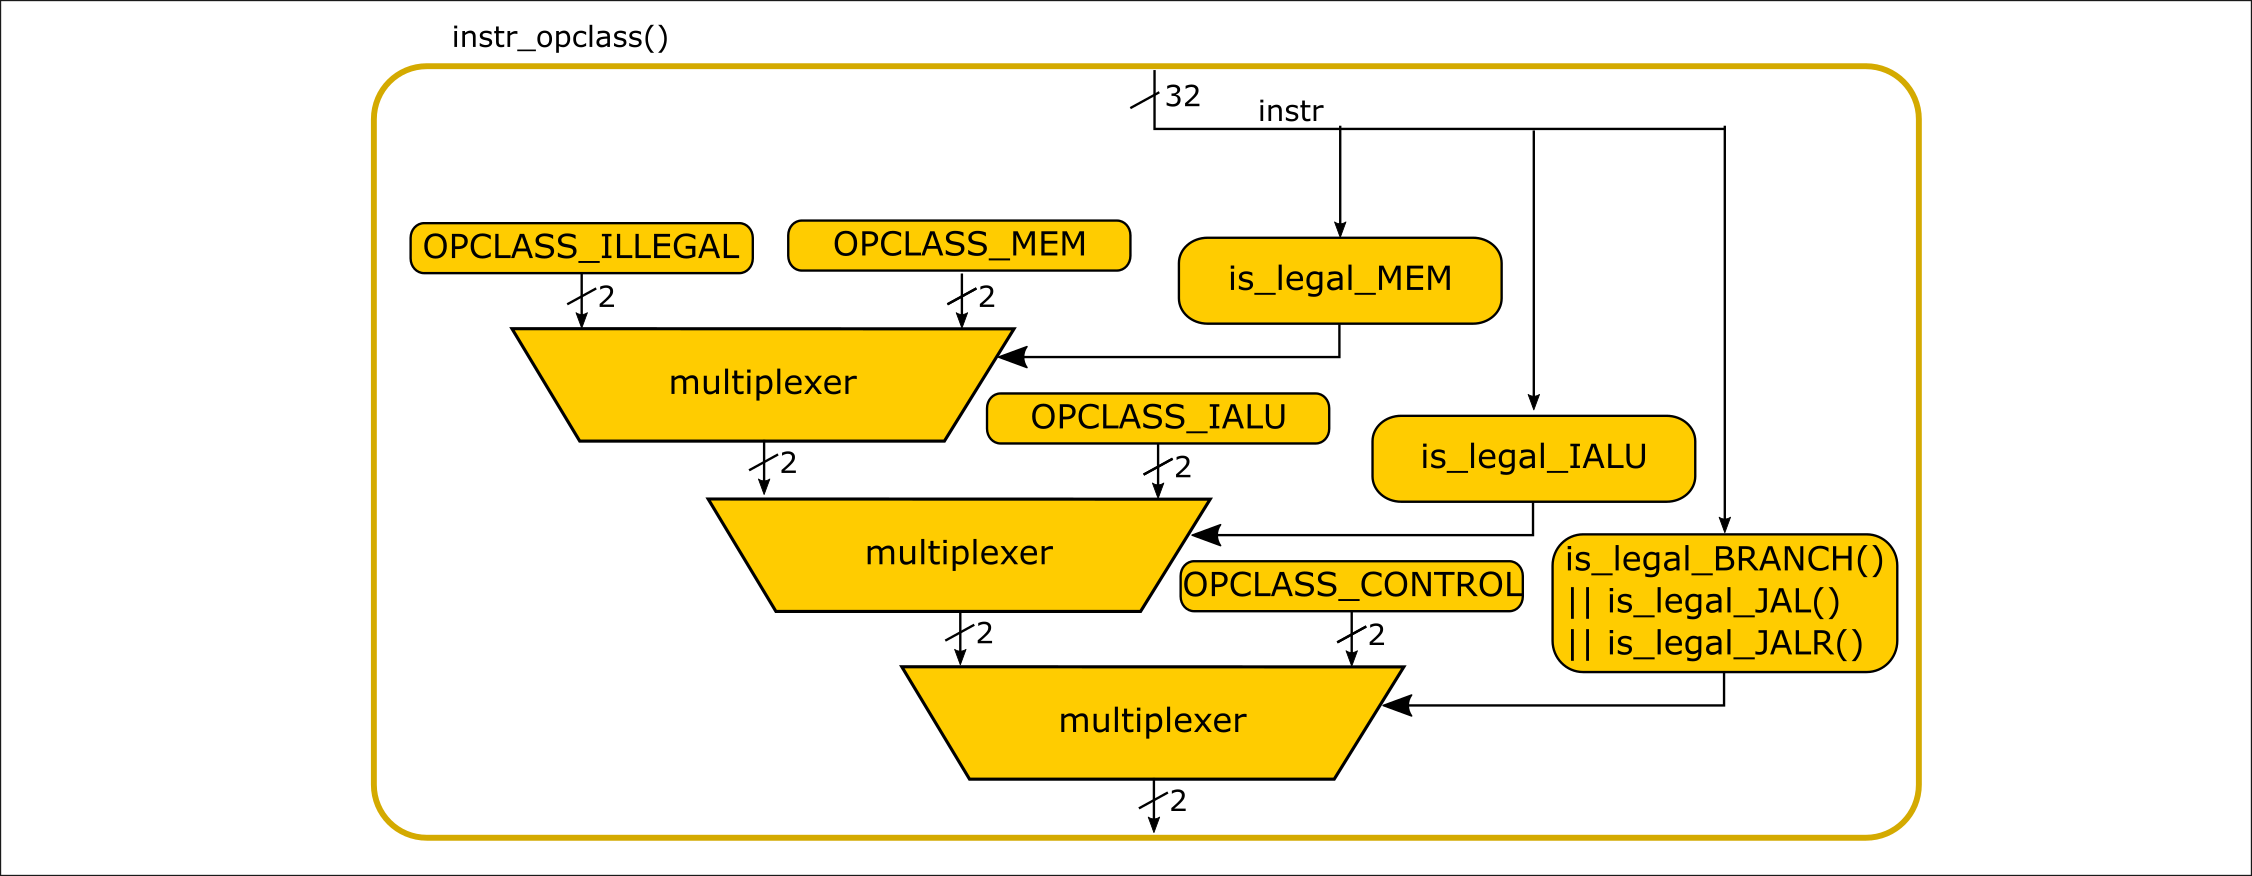
\includegraphics[width=6in,angle=0]{ch040_Combo_Circuits/Figures/Fig_Combo_Multiplexer_Cascade}}
  \caption{\label{Fig_Combo_Multiplexer_Cascade}Nested if-then-elses become cascaded multiplexers}
\end{figure}

% ================================================================

\subsection{Parallel multiplexers and MUX synthesis}

\index{BSV!multiplexers!parallel}

The circuit in Figure~\ref{Fig_Combo_Multiplexer_Cascade} has a
serial structure---the \verb|OPCLASS_CONTROL| branch has priority, and
only if its condition is False can one of the other results flow
through.  Also observe that the longest path length increases
\emph{linearly} with number of classes---here, \verb|OPCLASS_ILLEGAL|
flows through all three multiplexers.

But we know from RISC-V instruction encodings that the
\verb|OPCLASS_CONTROL|, \verb|OPCLASS_IALU| and \verb|OPCLASS_MEM|
conditions are \emph{mutually exclusive}; no instruction
simultaneously falls into more than one such class.  In such
situations (mutually exclusive conditions) it is possible to create
more a efficient circuit called a \emph{parallel MUX}.  An exercise
below shows how to create a parallel MUX explicitly, but in many cases
downstream RTL-to-lower-level-hardware synthesis tools will do this
automatically.

% ================================================================

\subsection{Exercises}

\begin{enumerate}

\item Write a testbench for the \verb|instr_opclass()| function: pass
  in different 32-bit instructions to produce the op class, and print
  out the op class.  When printing the class, try printing it as an
  integer, and also using \verb|fshow()|.

\item Write a new version of the \verb|instr_opclass()| function that
  expresses a parallel MUX instead of a priority MUX.  The key ideas
  are:

  \begin{itemize}

    \item Define a value \verb|x_CONTROL| that is either
      \verb|OPCLASS_CONTROL|, or 0 (of the same bit-width) if the
      \verb|Bool| values of \verb|is_legal_BRANCH()|,
      \verb|is_legal_JAL()| and \verb|is_legal_JALR()| are all False.
      We can implement this by replicating the 1-bit Bool condition to
      the width of the \verb|OpClass| type and bitwise-AND'ing this
      with \verb|OPCLASS_CONTROL|.

    \item Similarly, define values \verb|x_IALU| and \verb|x_MEM| that
       is either \verb|OPCLASS_IALU|/\verb|OPCLASS_MEM| or 0 if the
       \verb|Bool| value of
       \verb|is_legal_IALU()|/\verb|is_legal_MEM()| is False.

    \item Define a value \verb|x_ILLEGAL| that is either
      \verb|OPCLASS_ILLEGAL|, or 0 if any of
      the previous conditions is True.

    \item Finally, just bitwise-OR the four \verb|x_XXX|values
      together to produce there result.

  \end{itemize}

  This kind of MUX is also called an AND-OR mux because of its
  structure.  Note that it relies for correct operation on
  \emph{precisely one} of the bitwise-OR arguments being True.  Here,
  we are assured of this because of the mutual exclusivity of the
  conditions.

\item Sketch out a schematic diagram for the hardware of the parallel
  MUX in the previous exercise.

  The schematic will clearly reveal the parallel nature of the MUX
  compared to the serial nature of the priority MUX shown earlier in
  the schematic in Figure~\ref{Fig_Combo_Multiplexer_Cascade}.

  How many multiplexers does each \verb|OPCLASS_XXX| value flow
  through?  How many bitwise-OR operators are needed?  Note that we
  can organize the bitwise-OR operators as a balanced binary tree, so
  that the path through the circuit grows \emph{logarithmically}, not
  linearly, with the number of classes.

\item Test your new version of the \verb|instr_opclass()| function in
  your testbench.

\end{enumerate}

% ****************************************************************

\section{BSV: Sharing code for RV32 and RV64 {\via} parameterization}

\label{BSV_Paramterizing_XLEN}

\index{BSV!parameterization}

The RISC-V ISA is actually two ISAs---a 32-bit ISA called RV32 and a
64-bit ISA called RV64.  These are not randomly different ISAs; they
have been carefully engineered to overlap as much as possible:

\begin{itemize}

\item Most of the RV32 instructions are exactly the same in RV64

\item Three R32 instructions are slightly different in RV64--the shift
instructions SLLI, SRLI and SRAI have 5-bit shift-amounts in RV32
(allowing up to 32-bit shifts), whereas they have 6-bit shift-amounts
in RV64 (allowing up to 64-bit shifts).

\item RV64 adds several new instructions that compute on 64-bit values.

\end{itemize}

Because of this large overlap of RV32 and RV64, we would like to share
BSV code as much as possible between RV32 and RV64, {\ie} we would
like to parameterize our BSV code so that it can be re-used between
RV32 and RV64 implementations.

% ================================================================

\subsection{BSV: Numeric types}

\label{BSV_Numeric_types}

We have mentioned the type \verb|Bit#(n)| frequently so far,
representing bit-vectors of width \emph{n} bits.  All our examples
showed a particular \emph{n}, such as:

\begin{Verbatim}[frame=single, numbers=left]
   Bit #(32) instr;
   Bit #(32) pc_val;
\end{Verbatim}

The first declaration is fine for both RV32 and RV64, since
instructions are 32-bits wide in both.  However, the second
declaration only works in RV32, since the program counter is 64-bits
wide in RV64 (type \verb|Bit#(64)|).

\label{BSV_numeric_types}
\index{BSV!Types!numeric}

The ``32'' or ``64'' argument to the \verb|Bit#(n)| type is a
\emph{numeric type}.  Although syntactically they look just like the
\emph{values} 32 and 64, when used inside a type-expression like
\verb|Bit#(n)|, they are not values, but numeric types.  BSV's
type-system carefully distinguishes between these two cases because
numeric-types usually say something about \emph{hardware structure},
which cannot be changed once created!  So, while we can perform
arbitrary arithmetic on numeric \emph{values}, we cannot do so on
\emph{numeric types}.\footnote{A limited form of arithmetic is
possible on numeric types.  Consider a generic function that takes two
arguments of type {\tt Bit\#(m)} and {\tt Bit\#(n)} and returns the
concatenation of these bit-vectors: its output type is {\tt
Bit\#(m+n)}.  By limiting the available arithmetic \emph{bsc} can
resolve it completely ``statically'', {\ie} at compile time, before it
even compiles to Verilog RTL.  We ignore this for now, and discuss it
later.}

% ================================================================

\subsection{BSV: Type synonyms}

\label{BSV_Type_synonyms}

\index{BSV!type synonyms}
\index{BSV!Types!synonyms}

In BSV we can define a new symbolic name for an existing type, and
then we can use that symbolic names in place of the existing
type. Example, from RV32 code:

\begin{Verbatim}[frame=single, numbers=left]
   typedef 32 XLEN;      // new name for numeric type 32

   Bit #(XLEN) pc_val;
   Bit #(XLEN) rs1_val;  // Value read from register rs1 in register file
   Bit #(XLEN) rs2_val;  // Value read from register rs2 in register file
   Bit #(XLEN) rd_val;   // Value written to register rd in register file
\end{Verbatim}

By changing the single definition in line 1 to:
\begin{Verbatim}[frame=single, numbers=left]
   typedef 64 XLEN;      // new name for numeric type 32
\end{Verbatim}
the remaining code will work for RV64 as well.

% ================================================================

\subsection{BSV: The numeric value corresponding to a numeric type}

\label{BSV_value_of_numeric_type}

\index{BSV!valueOf: value of a numeric type}
\index{BSV!Types!valueOf: value of a numeric type}

Although BSV keeps a strict separation of numeric types and numeric
values (and limits the available arithmetic on the former), it is
always safe to convert a numeric type into the corresponding numeric
value, since these values are all known statically (at compile time).
The built-in pseudo-function \verb|valueOf()| is provided for this:

\begin{Verbatim}[frame=single, numbers=left]
   Integer xlen = valueOf (XLEN);
\end{Verbatim}

Here, \verb|xlen| is an ordinary value variable whose integer value is
the same as that expressed by the numeric type \verb|XLEN|.

% ================================================================

\subsection{BSV: Conditional compilation}

\label{BSV_Conditional_compilation}

\index{BSV!Conditional compilation}

Just like in Verilog, SystemVerilog and C/C++, the \emph{bsc} compiler
runs BSV source code through a ``pre-processor'' before compilation,
which can perform simple text (``macro'') substitutions.  Using this
facility, we can pass an argument to the compiler that has the effect
of configuring the source code for RV32 or RV64 (the following code is
from Fife/Magritte's \verb|Arch.bsv| file:

\begin{Verbatim}[frame=single, numbers=left]
`ifdef RV32

   typedef 32 XLEN;

`elsif RV64

   typedef 64 XLEN;

`endif

   Integer xlen = valueOf (XLEN);
\end{Verbatim}

As in Verilog and SystemVerilog, pre-processor directives begin with a
\verb|`| character (back-tick) (analogous to \verb|#ifdef| in the
C/C++ pre-processor).

When we invoke the \emph{bsc} compiler, we can pass it command line
arguments \verb|-DRV32| or \verb|-DRV64|; the pre-processor will then
select the appropriate \verb|typedef| line.  Thus, we can write common
code that will work for both RV32 and RV64.  The integer value
\verb|xlen| will have the numeric value 32 or 64 depending on how it
was compiled.

Pre-processor macros allow us to conditionally compile different
source text based on the macro definitions we supply to the compiler.
We can also compile alternatives based on the value \verb|xlen|

\begin{Verbatim}[frame=single, numbers=left]
   if (xlen == 32) begin
      ... code that must execute if we are in RV32 mode ...
   end
   else begin
      ... code that must execute if we are in RV64 mode ...
   end
\end{Verbatim}

Whenever possible, it is preferable to use the \verb|if(xlen==...)|
form instead of the \verb|`ifdef| form for conditional compilation
because (a), the code is more readable and (b), as we experience in
many languages, pre-processor macros can be quite dodgy (scoping,
inadvertant variable capture, inadvertant surprises due to
associativity of infix operators, ...).

Note that in the \verb|if(xlen==...)| form both arms of the
conditional must type-check correctly, whether \verb|xlen| is 32 or
64.  There are ways to achieve this with judicious use of bit-slicing,
\verb|extend()| and \verb|truncate()|; we will point them out as we
encounter them.  If the two arms cannot both type-check whether
\verb|xlen| is 32 or 64, we may have to resort to the \verb|`ifdef|
form.

There is zero run-time overhead in using the \verb|if(xlen==...)| form
because the \emph{bsc} compiler will evalute the if-condition
statically and reduce the if-then-else to just the relevant arm.

% ****************************************************************

\section{BSV: {\tt struct} types}

\label{BSV_struct_types}

\index{BSV!struct!type declaration}

In the Decode step of Figure~\ref{Fig_Simple_Instr_Exec} we
want to produce several results that will be passed on to subsequent
steps.  These include:

\begin{tightlist}

\item The PC.  This will be needed by BRANCH and AUIPC instructions to
  compute addresses that are offset from the current PC.  It will be
  needed in JAL instructions which save PC+4 or PC+2 as a
  return-address.  It will be needed for any traps (exceptions) that
  may occur, which save PC for the trap-handler.

\item The instruction, itself.  This will be needed for opcode
  details, the rs1, rs2 and rd register indexes, immediate values,
  {\etc}

\item The \verb|OpClass|.  This will be needed to dispatch the
  instruction to the appropriate handling step.

\item Whether the instruction reads rs1 and/or rs2 register values.
  This will be needed to control reading from the register file.

\item Whether the instruction writes an rd register value.  This will
  be needed to control writing to the register file.

\item The ``immediate'' value in the instruction, which is formatted
  differently depending on the class of instruction.

\end{tightlist}

This collection of values is most conveniently expressed as a
\verb|struct| type:

\begin{Verbatim}[frame=single, numbers=left]
typedef struct {Bit #(64)   inum;    // for debugging only
		Bit #(XLEN) pc;
		Bit #(32)   instr;

                OpClass     opclass;
		Bool        has_rs1;
		Bool        has_rs2;
		Bool        has_rd;
		Bit #(32)   imm;
} D_to_RR
deriving (Bits, FShow);
\end{Verbatim}

\index{BSV!deriving!Bits}

Because we said ``\verb|deriving(Bits)|'', the \emph{bsc} compiler
will automatically work out a representation for \verb|DD_to_RR|
values in bits, using the straightforward method of simply
concatenating the bit-vectors of each field into a bit-vector for the
whole struct.  If we had not said ``\verb|deriving(Bits)|'', we could
explicitly provide some other custom representation in bits.

\index{BSV!deriving!Fshow}

Because we said ``\verb|deriving(FShow)|'', the \emph{bsc} compiler
will automatically define an ``\verb|fshow()|'' function for this
type: if we print \verb|fshow(|\emph{v}\verb|)|, it will print
omething like this:

\begin{quote}\tt
DD\_to\_RR \{inum=..., pc=..., instr=..., ... \}
\end{quote}

% ================================================================

\subsection{Creating struct values}

\index{BSV!struct!entire struct values}

We can create a new value of type \verb|DD_to_RR| with syntax like
this:

\begin{Verbatim}[frame=single, numbers=left]
      DD_to_RR x = D_to_RR {inum:     ... value of field ...,
			    pc:       ... value of field ...,
			    instr:    ... value of field ...
			    ...};
\end{Verbatim}

The repetition of \verb|DD_to_RR| above seems verbose; the left-hand
side instance is the type, and the right-hand side instance is the
``struct constructor''. The \emph{bsc} compiler's type-analysis is
able to infer the type from the right-hand side, so we can just use
the keyword ``\verb|let|'':

\begin{Verbatim}[frame=single, numbers=left]
      let x = D_to_RR {inum:     ... value of field ...,
                       pc:       ... value of field ...,
		       instr:    ... value of field ...
		       ...};
\end{Verbatim}

% ================================================================

\subsection{Selecting struct fields}

\index{BSV!struct!field selection}

Struct fields can be selected using the usual ``dot'' notation common
to SystemVerilog and C/C++:

\begin{Verbatim}[frame=single, numbers=left]
x.pc
x.instr
\end{Verbatim}


% ================================================================

\subsection{Updating struct fields using assignment}

\index{BSV!struct!field assignment/update}

Struct fields can be updated with assignment using the usual ``dot''
notation common to SystemVerilog and C/C++:

\begin{Verbatim}[frame=single, numbers=left]
x.pc    = ... new value ...
x.instr = ... new value ...
\end{Verbatim}

% ****************************************************************

\section{RISC-V: The Decode function}

\label{Sec_Combo_Decode}

\index{Magritte!Decode function}

We are now in a position to write Figure~\ref{Fig_Simple_Instr_Exec}'s Decode function:

\begin{Verbatim}[frame=single, numbers=left]
function D_to_RR fn_D (Bit #(64) inum, Bit #(XLEN) instr, Bit #(32) instr);
   Bit #(5) rd = instr_rd (instr);

   // Baseline info to next stage
   let d_to_rr = D_to_RR {inum:     inum,
                          pc:       pc,
                          instr:    instr,

                          opclass:  OPCLASS_ILLEGAL,
                          has_rs1:  False,
                          has_rs2:  False,
                          has_rd:   False,
                          imm:      0};

   if (is_legal_LUI (instr) || is_legal_AUIPC (instr)) begin
      d_to_rr.opclass = OPCLASS_IALU;
      d_to_rr.has_rd  = (rd != 0);
      d_to_rr.imm     = zeroExtend (instr_imm_U (instr));
   end

   else if (is_legal_BRANCH (instr)) begin
      d_to_rr.opclass = OPCLASS_CONTROL;
      d_to_rr.has_rs1 = True;
      d_to_rr.has_rs2 = True;
      d_to_rr.imm     = zeroExtend (instr_imm_B (instr));
   end

   else if (is_legal_JAL (instr)) begin
      d_to_rr.opclass = OPCLASS_CONTROL;
      d_to_rr.has_rd  = (rd != 0);
      d_to_rr.imm     = zeroExtend (instr_imm_J (instr));
   end

   else if (is_legal_JALR (instr)) begin
      d_to_rr.opclass = OPCLASS_CONTROL;
      d_to_rr.has_rs1 = True;
      d_to_rr.has_rd  = (rd != 0);
      d_to_rr.imm     = zeroExtend (instr_imm_I (instr));
   end

   else if (is_legal_LOAD (instr)) begin
      d_to_rr.opclass = OPCLASS_MEM;
      d_to_rr.has_rs1 = True;
      d_to_rr.has_rd  = (rd != 0);
      d_to_rr.imm     = zeroExtend (instr_imm_I (instr));
   end

   else if (is_legal_STORE (instr)) begin
      d_to_rr.opclass = OPCLASS_MEM;
      d_to_rr.has_rs1 = True;
      d_to_rr.has_rs2 = True;
      d_to_rr.imm     = zeroExtend (instr_imm_S (instr));
   end

   else if (is_legal_OP_IMM (instr)) begin
      d_to_rr.opclass = OPCLASS_IALU;
      d_to_rr.has_rs1 = True;
      d_to_rr.has_rd  = (rd != 0);
   end

   else if (is_legal_OP (instr)) begin
      d_to_rr.opclass = OPCLASS_IALU;
      d_to_rr.has_rs1 = True;
      d_to_rr.has_rs2 = True;
      d_to_rr.has_rd  = (rd != 0);
   end

   return d_to_rr;
endfunction
\end{Verbatim}

Note the use of functions \verb|instr_imm_I()|, \verb|instr_imm_S()|,
\verb|instr_imm_B()|, \verb|instr_imm_U()| and \verb|instr_imm_J()|,
which extract the ``immediate'' field from a 32-bit instruction.  For
the different classes of instruction (I, S, B, U, J), the immediates
are coded differently, and have different widths.  These functions
decode the bits and zero-extend them to XLEN bits (the width of
\verb|d_to_rr.imm|).  Later, in the ``execute'' code for each
instruction, we will pick out the relevant bits out of the XLEN bits,
and zero-extend or sign-extend them as needed for the particular
instruction.

An exercise below suggests that you write the code for these
\verb|instr_imm_X| functions.

Observe that the entire \verb|fn_D()| function is just a (large)
combinational circuit---it is an acyclic composition of smaller
combinational circuits, many of which we've seen earlier.

% ================================================================

\subsection{Exercises}

\begin{enumerate}

\item Write the functions \verb|instr_imm_I()|, \verb|instr_imm_S()|,
  \verb|instr_imm_B()|, \verb|instr_imm_U()| and \verb|instr_imm_J()|.

\item Write a testbench for \verb|fn_D()|, apply it on a number of
  32-bit values (instructions) and print the results.

\end{enumerate}

% ****************************************************************
